% Options for packages loaded elsewhere
% Options for packages loaded elsewhere
\PassOptionsToPackage{unicode}{hyperref}
\PassOptionsToPackage{hyphens}{url}
\PassOptionsToPackage{dvipsnames,svgnames,x11names}{xcolor}
%
\documentclass[
  english,
  11pt,
]{article}
\usepackage{xcolor}
\usepackage[margin=1in]{geometry}
\usepackage{amsmath,amssymb}
\setcounter{secnumdepth}{-\maxdimen} % remove section numbering
\usepackage{iftex}
\ifPDFTeX
  \usepackage[T1]{fontenc}
  \usepackage[utf8]{inputenc}
  \usepackage{textcomp} % provide euro and other symbols
\else % if luatex or xetex
  \usepackage{unicode-math} % this also loads fontspec
  \defaultfontfeatures{Scale=MatchLowercase}
  \defaultfontfeatures[\rmfamily]{Ligatures=TeX,Scale=1}
\fi
\usepackage{lmodern}
\ifPDFTeX\else
  % xetex/luatex font selection
\fi
% Use upquote if available, for straight quotes in verbatim environments
\IfFileExists{upquote.sty}{\usepackage{upquote}}{}
\IfFileExists{microtype.sty}{% use microtype if available
  \usepackage[]{microtype}
  \UseMicrotypeSet[protrusion]{basicmath} % disable protrusion for tt fonts
}{}
\makeatletter
\@ifundefined{KOMAClassName}{% if non-KOMA class
  \IfFileExists{parskip.sty}{%
    \usepackage{parskip}
  }{% else
    \setlength{\parindent}{0pt}
    \setlength{\parskip}{6pt plus 2pt minus 1pt}}
}{% if KOMA class
  \KOMAoptions{parskip=half}}
\makeatother
% Make \paragraph and \subparagraph free-standing
\makeatletter
\ifx\paragraph\undefined\else
  \let\oldparagraph\paragraph
  \renewcommand{\paragraph}{
    \@ifstar
      \xxxParagraphStar
      \xxxParagraphNoStar
  }
  \newcommand{\xxxParagraphStar}[1]{\oldparagraph*{#1}\mbox{}}
  \newcommand{\xxxParagraphNoStar}[1]{\oldparagraph{#1}\mbox{}}
\fi
\ifx\subparagraph\undefined\else
  \let\oldsubparagraph\subparagraph
  \renewcommand{\subparagraph}{
    \@ifstar
      \xxxSubParagraphStar
      \xxxSubParagraphNoStar
  }
  \newcommand{\xxxSubParagraphStar}[1]{\oldsubparagraph*{#1}\mbox{}}
  \newcommand{\xxxSubParagraphNoStar}[1]{\oldsubparagraph{#1}\mbox{}}
\fi
\makeatother


\usepackage{longtable,booktabs,array}
\usepackage{calc} % for calculating minipage widths
% Correct order of tables after \paragraph or \subparagraph
\usepackage{etoolbox}
\makeatletter
\patchcmd\longtable{\par}{\if@noskipsec\mbox{}\fi\par}{}{}
\makeatother
% Allow footnotes in longtable head/foot
\IfFileExists{footnotehyper.sty}{\usepackage{footnotehyper}}{\usepackage{footnote}}
\makesavenoteenv{longtable}
\usepackage{graphicx}
\makeatletter
\newsavebox\pandoc@box
\newcommand*\pandocbounded[1]{% scales image to fit in text height/width
  \sbox\pandoc@box{#1}%
  \Gscale@div\@tempa{\textheight}{\dimexpr\ht\pandoc@box+\dp\pandoc@box\relax}%
  \Gscale@div\@tempb{\linewidth}{\wd\pandoc@box}%
  \ifdim\@tempb\p@<\@tempa\p@\let\@tempa\@tempb\fi% select the smaller of both
  \ifdim\@tempa\p@<\p@\scalebox{\@tempa}{\usebox\pandoc@box}%
  \else\usebox{\pandoc@box}%
  \fi%
}
% Set default figure placement to htbp
\def\fps@figure{htbp}
\makeatother



\ifLuaTeX
\usepackage[bidi=basic]{babel}
\else
\usepackage[bidi=default]{babel}
\fi
% get rid of language-specific shorthands (see #6817):
\let\LanguageShortHands\languageshorthands
\def\languageshorthands#1{}
\ifLuaTeX
  \usepackage[english]{selnolig} % disable illegal ligatures
\fi


\setlength{\emergencystretch}{3em} % prevent overfull lines

\providecommand{\tightlist}{%
  \setlength{\itemsep}{0pt}\setlength{\parskip}{0pt}}



 


\usepackage{fancyhdr}
\pagestyle{fancy}
\fancyhf{}
\fancyhead[L]{\leftmark}
\fancyhead[R]{\thepage}
\makeatletter
\@ifpackageloaded{caption}{}{\usepackage{caption}}
\AtBeginDocument{%
\ifdefined\contentsname
  \renewcommand*\contentsname{Table of contents}
\else
  \newcommand\contentsname{Table of contents}
\fi
\ifdefined\listfigurename
  \renewcommand*\listfigurename{List of Figures}
\else
  \newcommand\listfigurename{List of Figures}
\fi
\ifdefined\listtablename
  \renewcommand*\listtablename{List of Tables}
\else
  \newcommand\listtablename{List of Tables}
\fi
\ifdefined\figurename
  \renewcommand*\figurename{Figure}
\else
  \newcommand\figurename{Figure}
\fi
\ifdefined\tablename
  \renewcommand*\tablename{Table}
\else
  \newcommand\tablename{Table}
\fi
}
\@ifpackageloaded{float}{}{\usepackage{float}}
\floatstyle{ruled}
\@ifundefined{c@chapter}{\newfloat{codelisting}{h}{lop}}{\newfloat{codelisting}{h}{lop}[chapter]}
\floatname{codelisting}{Listing}
\newcommand*\listoflistings{\listof{codelisting}{List of Listings}}
\makeatother
\makeatletter
\makeatother
\makeatletter
\@ifpackageloaded{caption}{}{\usepackage{caption}}
\@ifpackageloaded{subcaption}{}{\usepackage{subcaption}}
\makeatother
\usepackage{bookmark}
\IfFileExists{xurl.sty}{\usepackage{xurl}}{} % add URL line breaks if available
\urlstyle{same}
\hypersetup{
  pdftitle={Session 11: Hands-on Activity},
  pdfauthor={Masaki EGUCHI, Ph.D.},
  pdflang={en},
  colorlinks=true,
  linkcolor={blue},
  filecolor={Maroon},
  citecolor={Blue},
  urlcolor={Blue},
  pdfcreator={LaTeX via pandoc}}


\title{Session 11: Hands-on Activity}
\author{Masaki EGUCHI, Ph.D.}
\date{}
\begin{document}
\maketitle


\section{Housekeeping}\label{housekeeping}

\section{Session overview}\label{session-overview}

\subsection{🎯 Learning Objectives}\label{learning-objectives}

By the end of this session, students will be able to:

\begin{quote}
\begin{itemize}
\tightlist
\item
  Understand NLP tasks such as POS tagging and dependency parsing
\item
  Understand how automated parsing works
\item
  Conduct multi-lingual Part-Of-Speech (POS) tagging using TagAnt
\item
  Conduct POS tagging using spaCy library in Python (through Google
  Colab)
\item
  Conduct Dependency parsing using spaCy library in Python (through
  Google Colab)
\end{itemize}
\end{quote}

\begin{center}\rule{0.5\linewidth}{0.5pt}\end{center}

\subsection{Hands-on Activity}\label{hands-on-activity}

\textbf{Task 1}: POS tagging with TagAnt

\textbf{Task 2}: POS-sensitive frequency list

\textbf{Task 3}: Understanding dependency grammar through visualization

\subsection{POS tagging with TagAnt}\label{pos-tagging-with-tagant}

\subsection{Tagging with TagAnt}\label{tagging-with-tagant}

\begin{enumerate}
\def\labelenumi{\arabic{enumi}.}
\tightlist
\item
  Open TagAnt
\item
  Select \texttt{Input\ Files}
\item
  Select \texttt{Language}
\item
  Select Display information (see next)
\end{enumerate}

\subsection{Display setting info in
TagAnt}\label{display-setting-info-in-tagant}

Followings are basic selection in TagAnt.

\begin{longtable}[]{@{}lll@{}}
\toprule\noalign{}
Menu & Function & Example \\
\midrule\noalign{}
\endhead
\bottomrule\noalign{}
\endlastfoot
word & tokenization & dogs, ran \\
pos & POS tag (simple) & NOUN, VERB \\
pos\_tag & POS tag (detailed) & NNS, VBD \\
lemma & lemmatized word & dog, run \\
\end{longtable}

\subsection{Other Diaplay settings}\label{other-diaplay-settings}

\begin{longtable}[]{@{}lll@{}}
\toprule\noalign{}
Menu & Function & Example \\
\midrule\noalign{}
\endhead
\bottomrule\noalign{}
\endlastfoot
word+pos & tokenization and POS & dogs\_NOUN, ran\_VERB \\
word+lemma +pos\_tag & token+lemma+POS & dogs\_dog\_NN,
ran\_run\_VERB \\
\end{longtable}

\subsection{Task 1: Annotating Japanese text (10
mins)}\label{task-1-annotating-japanese-text-10-mins}

\begin{itemize}
\tightlist
\item
  Annotate 50 Japanese text files with TagAnt.
\item
  Create frequency list for \texttt{aozora\_50}
\end{itemize}

\subsection{Task 1: Answer}\label{task-1-answer}

\textbf{Before}

\begin{verbatim}
「大溝」

 僕は本所界隈のことをスケツチしろといふ社命を受け、同じ社のO君と一しよに久振りに本所へ出かけて行つた。
\end{verbatim}

\textbf{After}

\begin{verbatim}
「_補助記号-括弧開_「 大溝_名詞-固有名詞-人名-姓_大溝 」_補助記号-括弧閉_」

 _SPACE_  僕_代名詞_僕 は_助詞-係助詞_は 本所_名詞-固有名詞-地名-一般_本所 界隈_名詞-普通名詞-一般_界隈 の_助詞-格助詞_の こと_名詞-普通名詞-一般_こと を_助詞-格助詞_を スケツチ_名詞-普通名詞-一般_スケツチ しろ_動詞-非自立可能_する と_助詞-格助詞_と いふ_動詞-一般_いふ 社命_名詞-普通名詞-一般_社命 を_助詞-格助詞_を 受け_動詞-一般_受ける 、_補助記号-読点_、 同じ_連体詞_同じ 社_名詞-普通名詞-助数詞可能_社 の_助詞-格助詞_の O_名詞-普通名詞-一般_o 君_接尾辞-名詞的-一般_君 と_助詞-格助詞_と 一しよ_名詞-普通名詞-サ変可能_一しよ に_助詞-格助詞_に 久_形容詞-一般_久い 振り_接尾辞-名詞的-一般_振り に_助詞-格助詞_に 本所_名詞-固有名詞-地名-一般_本所 へ_助詞-格助詞_へ 出_動詞-一般_出る かけ_動詞-非自立可能_かける て_助詞-接続助詞_て 行つ_動詞-一般_行ふ た_助動詞_た 。_補助記号-句点_。
\end{verbatim}

\begin{center}\rule{0.5\linewidth}{0.5pt}\end{center}

\subsection{Task 2: Frequency-list by POS tags (10
mins)}\label{task-2-frequency-list-by-pos-tags-10-mins}

\begin{itemize}
\tightlist
\item
  Using \texttt{AntConc}, create following frequency lists:

  \begin{itemize}
  \tightlist
  \item
    Create a frequency list of \texttt{動詞-非自立可能}
  \end{itemize}
\item
  If you are done, please create another frequency list with different
  search terms.
\end{itemize}

\subsection{Task 2: Key}\label{task-2-key}

\begin{figure}[H]

{\centering \pandocbounded{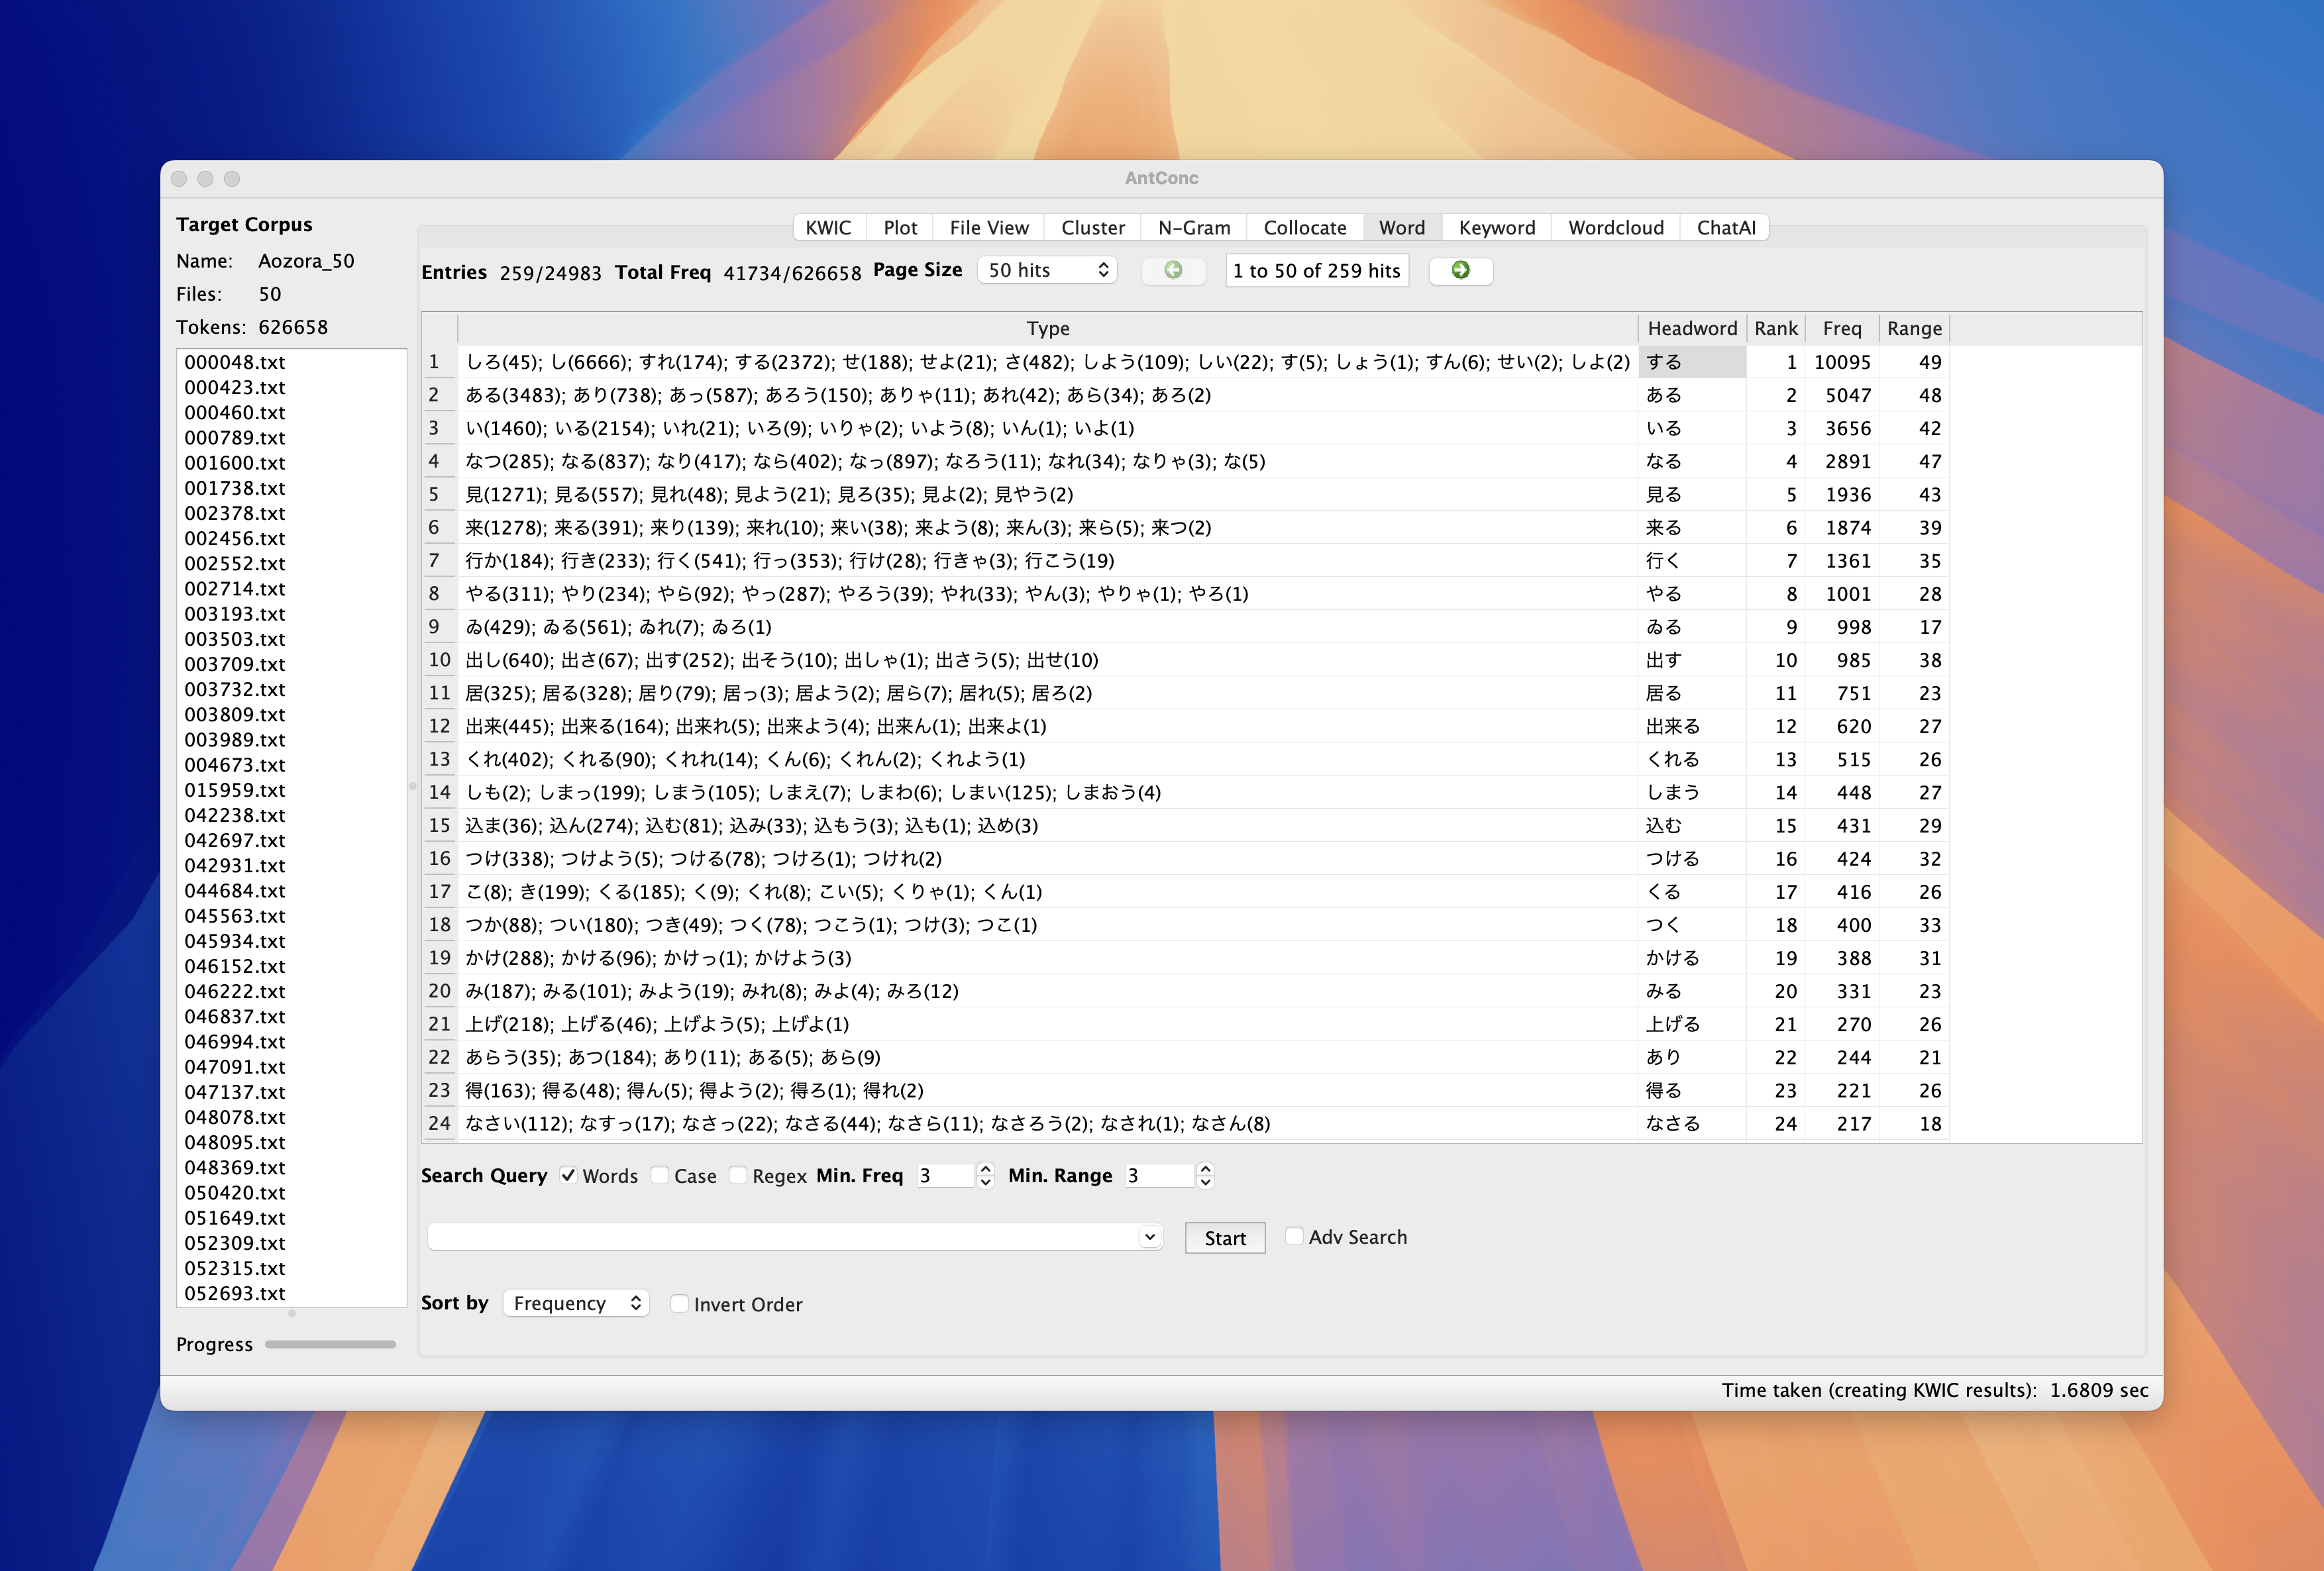
\includegraphics[keepaspectratio]{../../assets/session-11/非自立可能動詞.png}}

}

\caption{非自立可能動詞}

\end{figure}%

\subsection{Advanced options in
TagAnt}\label{advanced-options-in-tagant}

\begin{itemize}
\tightlist
\item
  In TagAnt, you can download models for other languages.
\end{itemize}

\begin{figure}[H]

{\centering \pandocbounded{\includegraphics[keepaspectratio]{../../assets/session-11/tagant-advanced.gif}}

}

\caption{loading other models}

\end{figure}%

\subsection{Any questions?}\label{any-questions}

\begin{itemize}
\tightlist
\item
  Now you can parse multilingual text with TagAnt.
\end{itemize}

\begin{center}\rule{0.5\linewidth}{0.5pt}\end{center}

\section{Understanding dependency
grammar}\label{understanding-dependency-grammar}

\subsection{Goals}\label{goals}

\begin{itemize}
\tightlist
\item
  Describe grammatical structure of a simple sentence using terminology
  such as \texttt{ROOT},\texttt{head}, \texttt{dependency\ type}, and
  \texttt{dependent}.
\end{itemize}

\subsection{Dependency grammar
(係受け)}\label{dependency-grammar-ux4fc2ux53d7ux3051}

\begin{itemize}
\tightlist
\item
  Dependency grammar is particular type of syntactic tree.
\item
  forms a tree by defining binary relations between running tokens.
\item
  Each token in the sentence is governed by one token (i.e.,
  \texttt{head})
\item
  The highest in the syntactic tree is termed as \texttt{ROOT}
\end{itemize}

\subsection{Dependency grammar (係受け) -
2}\label{dependency-grammar-ux4fc2ux53d7ux3051---2}

\begin{itemize}
\tightlist
\item
  There are a few different approaches to formalize dependency

  \begin{itemize}
  \tightlist
  \item
    Universal Dependency
  \item
    Stanford Dependency
  \item
    ClearNLP
  \item
    etc.
  \end{itemize}
\end{itemize}

\subsection{Simple example}\label{simple-example}

The following is a dependency for \texttt{I\ play\ baseball}.

\begin{figure}[H]

{\centering \pandocbounded{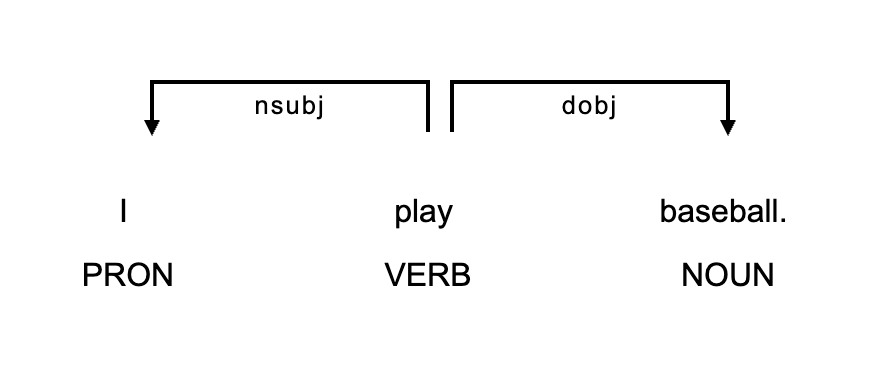
\includegraphics[keepaspectratio]{../../assets/session-11/dep-1.png}}

}

\caption{simple-dependency}

\end{figure}%

\subsection{In table format}\label{in-table-format}

The same sentence, \texttt{I\ play\ baseball} can be expressed in the
following format

\begin{longtable}[]{@{}llll@{}}
\toprule\noalign{}
tid & token & dep & head \\
\midrule\noalign{}
\endhead
\bottomrule\noalign{}
\endlastfoot
1 & I & nsubj & 2 \\
2 & play & ROOT & \\
3 & baseball & dobj & 2 \\
4 & . & punct & 2 \\
\end{longtable}

This type of vertical format is often used to represent multi-layered
token information.

\subsection{Some excercise - Problem
1}\label{some-excercise---problem-1}

Try filling in the gap in the following table.

\begin{longtable}[]{@{}llll@{}}
\toprule\noalign{}
tid & token & dep & head \\
\midrule\noalign{}
\endhead
\bottomrule\noalign{}
\endlastfoot
1 & I & & \\
2 & love & ROOT & \\
3 & beef & & \\
4 & tongue & & \\
5 & . & punct & 2 \\
\end{longtable}

\subsection{Some excercise - Problem
2}\label{some-excercise---problem-2}

Try filling in the gap in the following table.

\begin{longtable}[]{@{}llll@{}}
\toprule\noalign{}
tid & token & dep & head \\
\midrule\noalign{}
\endhead
\bottomrule\noalign{}
\endlastfoot
1 & The & & \\
2 & cat & & \\
3 & sleeps & ROOT & \\
4 & on & & \\
5 & the & & \\
6 & mat & & \\
7 & . & punct & 3 \\
\end{longtable}

\subsection{Some excercise - Problem
3}\label{some-excercise---problem-3}

Try filling in the gap in the following table.

\begin{longtable}[]{@{}llll@{}}
\toprule\noalign{}
tid & token & dep & head \\
\midrule\noalign{}
\endhead
\bottomrule\noalign{}
\endlastfoot
1 & She & & \\
2 & quickly & & \\
3 & reads & ROOT & \\
4 & interesting & & \\
5 & books & & \\
6 & . & punct & 3 \\
\end{longtable}

\subsection{Let's parse the sentence.}\label{lets-parse-the-sentence.}

\begin{itemize}
\item
  Visit our
  \href{https://huggingface.co/spaces/egumasa/simple-text-analyzer}{webapp}
\item
  Try the sentences above and analyze their dependencies
\end{itemize}

\subsection{Questions?}\label{questions}

\section{Reflection}\label{reflection}

\section{Next step}\label{next-step}




\end{document}
